\subsection{Boltzmann Transport and Chambers Formula for Optical Conductivity}
The Boltzmann transport equation is a semi-classical model of flow 
which gives a more detailed model of the electronic properties of a material, 
since it accounts for the trajectories of the electrons in phase space. 
Chambers' formula thus describes the real electronic structure of the material, 
and can thus account for anisotropic scattering processes.

Using the Boltzmann equation, with a few reasonable assumptions, 
one can derive the Chambers formula for conductivity. 
The formula is usually applied for DC conductivity ($\sigma(\omega=0)$), 
but it can be generalized for optical conductivity too (see appendix \ref{sec:chambers}).
This model has been used successfully in the past to study the behavior of cuprates 
and make predictions about their physical properties\cite{grissonnanche2021, grissonnanche2024, fang2022, gourgout2022, ataei2022}, 
justifying its use here.

According to the Chambers formula for optical conductivity, 
the conductivity tensor in the cartesian basis is then given by :
\begin{equation}
	\sigma_{ab} = \frac{2e^2}{(2\pi)^d\hbar}\int_{\mathrm{FS}}\dd{\vb{k}}\hat{v}_a(\vb{k})
        \int_0^{\infty}\dd{t}v_b(\vb{k}(t))\exp{i\omega t
        - \int_0^t \frac{\mathop{dt'}}{\tau(\vb{k}(t'))}}
\end{equation}
where $\mathrm{FS}$ is the Fermi surface, $d$ is the number of dimensions of the system, $\vb{k}$ is the
wavevector, $\omega$ is the frequency of the electromagnetic waves, $v_b$ is the veclocity of the
charge carriers in the $b$ direction, $\hat{v}_a\equiv v_a/\abs{\vb{v}}$, and $\tau$ is the
relaxation time (inverse of the scattering rate). 

We can have an intuitive understanding of this formula. 
First, as we see here, we are only interested in the electrons that live on (or near, strictly speaking when at nonzero temperature) the Fermi surface as defined previously. 
Indeed, it is possible to show, as was mentioned above, that only they will meaningfully contribute to conduction. 
For any starting point $\vb{k}$ on the Fermi surface (first integral) with a given associated velocity in the $a$ component, 
we are interested the electron's velocity in the $b$ component along its trajectory (parametrised by $t$,  which can be time). 
The exponential terms account for the influence of the varying electrical field and the scattering rate of electron (that is not uniform in phase space). 
The magnetic field appears implicitly in the movement equations that define $\b{k}(t)$.

Thus, the formula reflects how, on average, electrons move in the $b$ direction when initially excited in the $a$ direction.


In order to evaluate the integral, we should then couple it with :
\begin{enumerate}
    \item a movement equation;
    \item a model for the scattering rate;
    \item the shape of the Fermi surface.
\end{enumerate}

In the following, 
we explain in more detail the different components and the methods of evaluating this formula.

\subsubsection{Movement Equation}
Since we are only interested in the first order response of the system to an electric field, we
can solve the movement equation with only a magnetic field. That is,
\begin{empheq}[left=\empheqlbrace]{align}
    \hbar\dv{\vb{k}}{t} &= e\vb{v}\times\vb{B}, \\
    \vb{v} &= \frac{1}{\hbar}\grad_{\vb{k}}\varepsilon(\vb{k}),
\end{empheq}
Where $\varepsilon$ is the energy of the charge carriers. The movement equation can be solved
numerically for a discretization of the Fermi surface (since the Chambers formula integral is
evaluated over the Fermi surface).

Here, note that the magnetic field $\vb{B}$ is always pointed along the $z$ direction for the data
we examined. However, our methods allow any direction for the magnetic field too.

\subsubsection{Scattering Rate}
Following Grissonnanche et al.\cite{grissonnanche2021}, we used a simple model for the scattering
rate, respecting the symmetry of the system. It is given by
\begin{equation}
    \frac{1}{\tau(\vb{k})} = \Gamma(\vb{k}) = \Gamma_0 + \Gamma_k\abs{\cos(2\varphi)}^\nu,
\end{equation}
where $\varphi$ is the angle between the wavevector and the $k_x$ axis and $\Gamma_0$, $\Gamma_k$,
and $\nu$ are adjustable parameters. The shape of the scattering rate dependence is shown in figure \ref{fig:log_scattering}

\begin{figure}
    \centering
    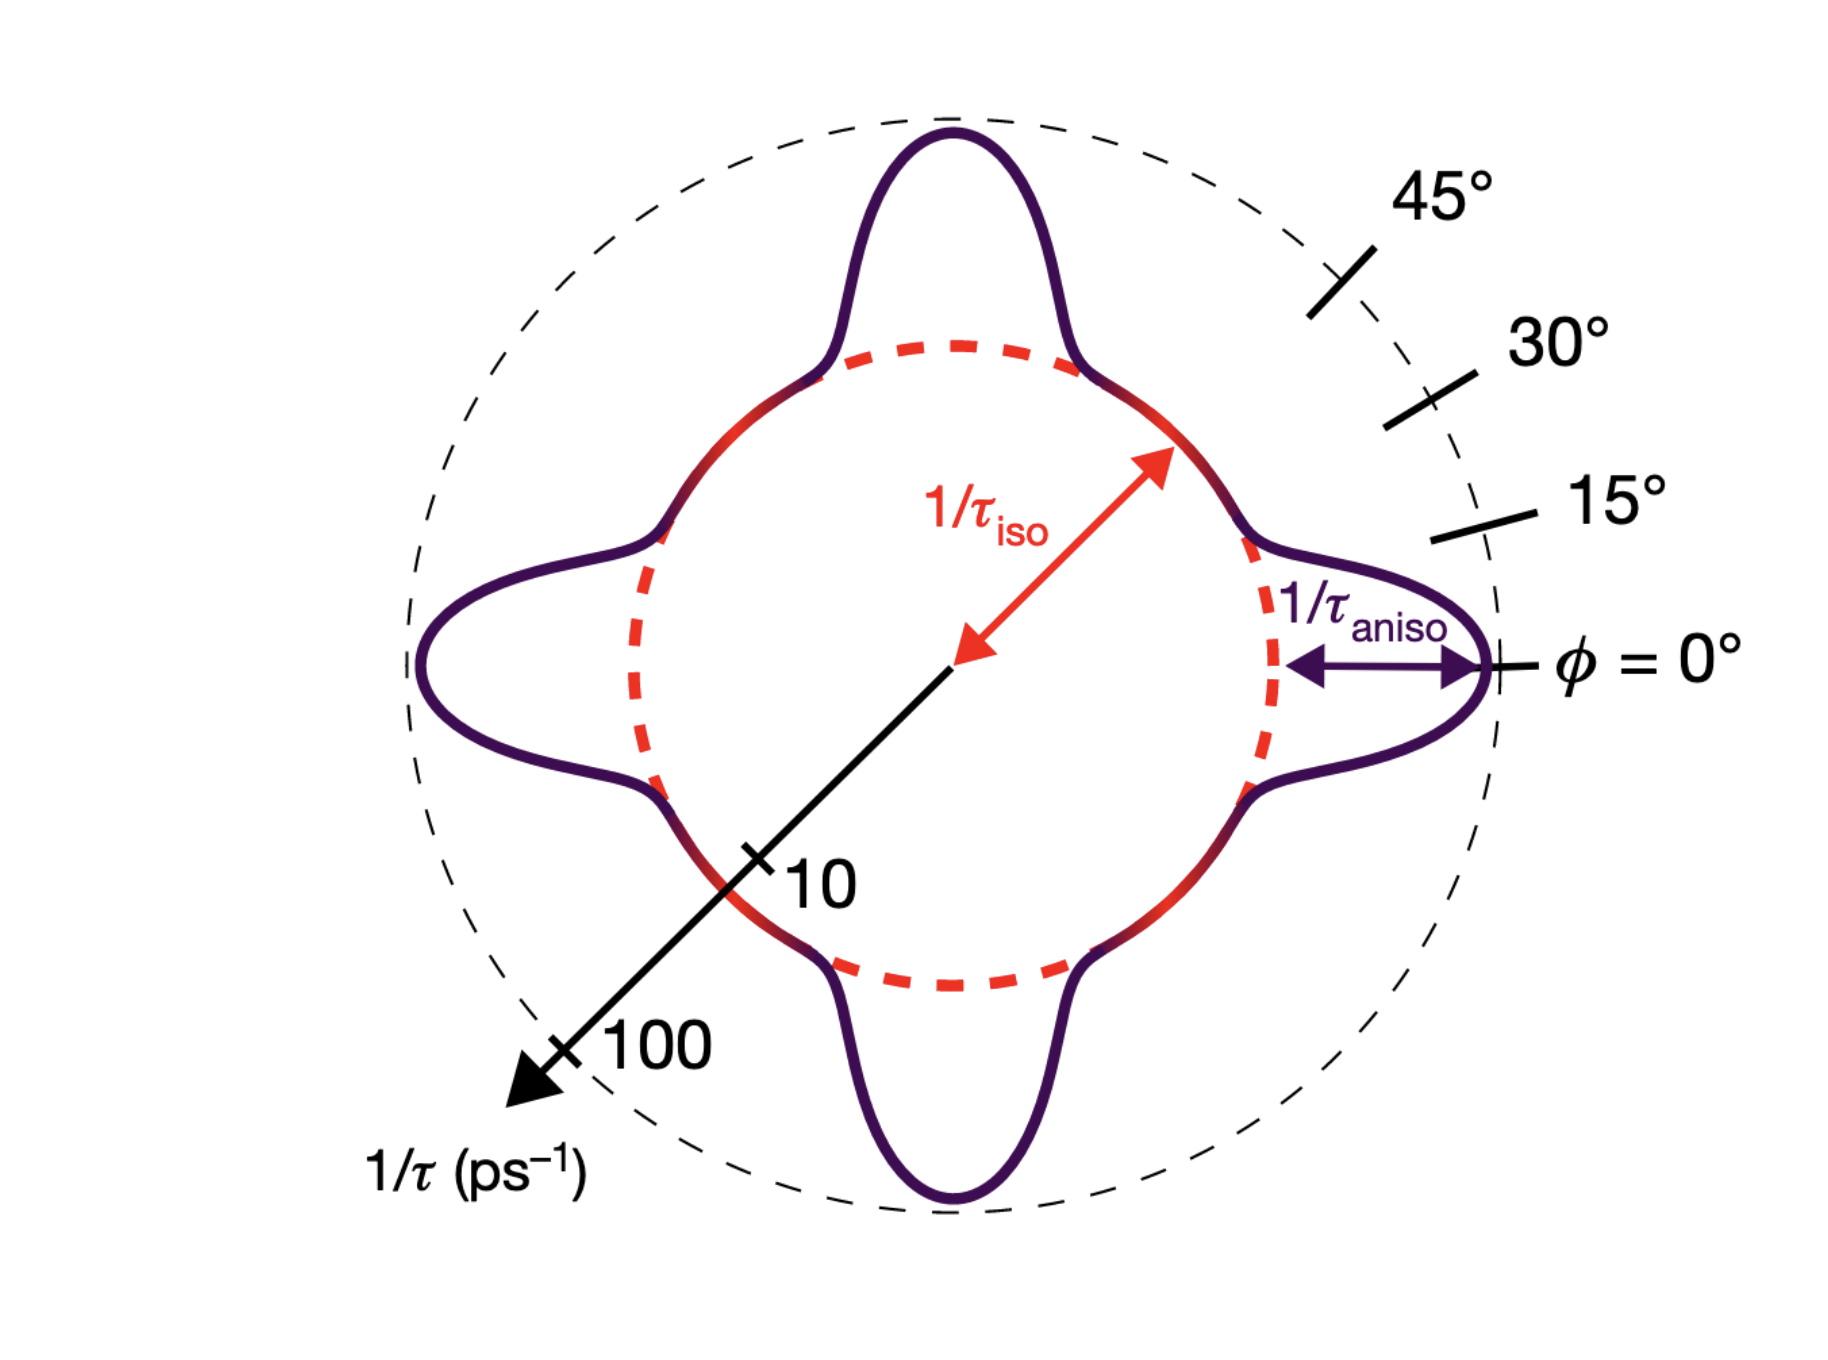
\includegraphics[width=0.7\textwidth]{figures/polar_log_scattering.png}
    \caption{(from Grissonnanche et al.\cite{grissonnanche2021}) Polar plot of the scattering rate $\Gamma(\vb{k})$ given by the model we used, on a logarithmic scale.}
    \label{fig:log_scattering}
\end{figure}


\subsubsection{Fermi Surface}
For the shape of the Fermi surface, we used a simple 3D tight-binding model for the Body centered
tetragonal crystal structure of LSCO, given by :
\begin{equation}
\begin{aligned}
    \varepsilon(\vb{k}) = &-\mu - 2t(\cos(k_x a) + \cos(k_y a)) \\
        &- 4t'\cos(k_x a)\cos(k_y a) - 2t''(\cos(2k_x a) + \cos(2k_y a)) \\
        &- 2t_z\cos(k_x a / 2)\cos(k_y a / 2)\cos(k_z c / 2)[\cos(k_x a) - \cos(k_y a)]^2,
\end{aligned}
\end{equation}
where $\mu$ is the chemical potential, $t$, $t'$, and $t''$ are the first, second, and third
nearest-neighbor hopping parameters, $t_z$ is the interlayer hopping parameter,
$a=3.75\angstrom$ is the in-plane lattice constant, and $c/2=6.6\angstrom$ is the
$\mathrm{CuO_2}$ layer spacing. These parameters are derived experimentally from ARPES measurements\cite{horio2018}. \\

With this new formalism, we can now set out to use the Chambers formula to analyze the optical conductivity data produced by Legros et al.\cite{legros2022} and extract $m_c \approx m^*$.
Our goal is then to see if our new $m_c$ still contradicts the effective mass obtained from specific heat. 
